%%%%%%%%%%%%%%%%%%%%%%%%%%%%%%%%%%%%%%%%%%%%%%%%%%%%%%%%%%%%%%%%%%%%%%%%
% Plantilla TFG/TFM
% Escuela Politécnica Superior de la Universidad de Alicante
% Realizado por: Jose Manuel Requena Plens
% Contacto: info@jmrplens.com / Telegram:@jmrplens
%%%%%%%%%%%%%%%%%%%%%%%%%%%%%%%%%%%%%%%%%%%%%%%%%%%%%%%%%%%%%%%%%%%%%%%%

\chapter{Introducción}

La gestión y recuperación eficiente de la información digital se ha convertido en un desafío cotidiano en la era de la sobrecarga informativa. Los volúmenes de datos personales y profesionales que almacenamos en nuestros dispositivos crecen exponencialmente, mientras que las herramientas tradicionales de búsqueda a menudo resultan insuficientes para localizar archivos específicos de manera rápida y precisa. Este proyecto se adentra en esta problemática, proponiendo una solución innovadora basada en los avances recientes en \gls{ia} y sistemas de Generación Aumentada por Recuperación (\gls{rag}).

\section{Panorama Actual: Desafíos en la Recuperación de Información}
Los métodos que se suelen usar para buscar y organizar archivos digitales dependen mucho de lo que se conoce como ``metadatos explícitos''. Estos se basan en información como el nombre del archivo, su fecha, o etiquetas que añadimos manualmente. Pero, esta forma de trabajar presenta varios inconvenientes:
\begin{itemize}
\item  \textbf{Insuficiencia de los metadatos tradicionales:} Muchas veces, los metadatos son inexistentes, incompletos o especifican fielmente el contenido real del archivo.
\item  \textbf{Falta de precisión en las búsquedas:} Las búsquedas basadas en palabras clave pueden ser ambiguas y no siempre manejan correctamente la intención del usuario, lo que lleva a resultados irrelevantes o a la omisión de la información que el usuario desea encontrar.
\end{itemize}
Con la llegada de la inteligencia artificial \gls{ia}, se abren nuevas puertas para mejorar cómo encontramos y manejamos nuestra información. La IA podría permitirnos buscar archivos de formas mucho más intuitivas, por ejemplo, entendiendo el contenido de una imagen o el tema de un documento sin necesidad de que nosotros le hayamos puesto etiquetas antes. Esto sería un gran avance respecto a los métodos tradicionales.

Sin embargo, aunque la inteligencia artificial nos da nuevas herramientas, también trae consigo sus propios retos. A veces, estos sistemas de IA pueden no ser lo suficientemente exactos para ciertas tareas. En el caso de las IA que generan contenido, como texto o imágenes, a veces pueden "alucinar", es decir, inventar información que parece correcta pero que en realidad no lo es. Además, la forma en que se entrena a un modelo de IA puede influir en cómo interpreta un archivo, pudiendo llevar a resultados que no son justos o que incluso discriminan a ciertos grupos. Esto, por supuesto, nos hace pensar en temas éticos importantes que hay que considerar.

Otro aspecto fundamental son los riesgos de seguridad y privacidad. Al guardar nuestros archivos en ``la nube'' (servidores de internet) y usar la IA para que nos ayude a organizarlos y entenderlos, estamos creando nuevas posibles vulnerabilidades. Estos sistemas pueden ser atacados por gente que quiera acceder sin permiso, robar datos o realizar ciberataques, tanto en el lugar donde se guardan los archivos como en los propios sistemas de IA. La información sensible de nuestros archivos, o incluso la información que la IA genera sobre ellos, podría quedar expuesta, ser modificada o perderse. Esto se vuelve especialmente grave cuando se trata de datos confidenciales o personales. Un fallo de seguridad en estos casos no solo significa perder información valiosa, sino que también puede traer serias consecuencias legales, problemas económicos y, si se trata de una empresa, dañar mucho su reputación.

Este contexto muestra la necesidad de sistemas más inteligentes y contextuales capaces de comprender el contenido de los archivos de forma más profunda, más allá de sus metadatos superficiales, y que al mismo tiempo garanticen la integridad y confidencialidad de la información.

\section{Avances Tecnológicos Fundamentales}
Para abordar los desafíos mencionados, este proyecto se apoya en los desarrollos más recientes en el campo de la Inteligencia Artificial, particularmente en las siguientes áreas:

\subsection{Inteligencia Artificial Multimodal: Convergencia de Lenguaje y Visión}
La \gls{ia} ha experimentado avances exponenciales, especialmente con el auge del \gls{nlp} y la Visión Artificial. La multimodalidad representa la capacidad de los sistemas de \gls{ia} para procesar, comprender y generar información a partir de múltiples tipos de datos o ``modalidades'' simultáneamente, como texto, imágenes, audio y vídeo.
\begin{itemize}
    \item \textbf{Procesamiento del Lenguaje Natural (\gls{nlp}):} Permite a las máquinas comprender, interpretar y generar lenguaje humano. Los \gls{llm}, como \gls{gpt} y sus variantes, han revolucionado este campo, demostrando una capacidad asombrosa para entender el contexto, generar texto coherente e incluso razonar sobre la información proporcionada.
    \item \textbf{Visión Artificial:} Es la disciplina que permite a las máquinas ``ver'' e interpretar el contenido de imágenes y vídeos. Implica tareas como la detección de objetos, el reconocimiento facial, la segmentación de imágenes y la generación de descripciones visuales.
    \item \textbf{Modelos Multimodales}: Hay modelos como \gls{clip} de OpenAI\footnote{Más información sobre \gls{clip} de OpenAI disponible en: \url{https://openai.com/es-ES/index/clip/}}, que son un gran ejemplo de cómo se juntan el lenguaje y la visión. \gls{clip} aprende a relacionar imágenes con las palabras que las describen. Gracias a esto, podemos buscar una imagen escribiendo lo que queremos encontrar, por ejemplo, ``un perro jugando en la playa'', y el sistema entiende qué buscar, o al revés. Para lograrlo, se entrena un sistema que codifica imágenes y otro que codifica texto, enseñándoles a encontrar las parejas correctas entre millones de imágenes y sus descripciones.
\end{itemize}

\subsection{Optimización de Modelos: Cuantización y Modelos Ligeros}
Para la aplicación práctica de estos modelos, sobre todo en dispositivos como el teléfono móvil, es muy importante considerar su eficiencia.
\begin{itemize}
    \item \textbf{Modelos Cuantizados:} La cuantización es un proceso que reduce la precisión numérica de los pesos y activaciones de un modelo de red neuronal, por ejemplo, de punto flotante de 32 bits a enteros de 8 bits. Esto disminuye significativamente el tamaño del modelo y acelera la inferencia, con una pérdida de precisión a menudo mínima. Esto es muy útil para que modelos grandes se puedan ejecutar en dispositivos de pocos recursos a cambio de perder un poco de precisión.
    \item \textbf{Modelos Ligeros (Lightweight Models):} Son arquitecturas de redes neuronales diseñadas específicamente para ser computacionalmente eficientes y tener un tamaño reducido, facilitando su despliegue en dispositivos móviles o embebidos sin sacrificar excesivamente el rendimiento.
\end{itemize}

\subsection{Sistemas de Generación Aumentada por Recuperación (\gls{rag})}
La Generación Aumentada por Recuperación (\gls{rag}) es una técnica que mejora el rendimiento de los \gls{llm} al conectarlos con fuentes de conocimiento externas. En lugar de depender solo de la información aprendida durante su entrenamiento, un sistema \gls{rag} funciona en dos pasos:
\begin{enumerate}
    \item \textbf{Recuperación (Retrieval):} Dada una consulta del usuario, el sistema primero busca y recupera fragmentos de información relevante de una base de datos, un conjunto de documentos o un corpus de conocimiento. Esta base de datos puede estar compuesta por embeddings (representaciones vectoriales densas) del contenido de los archivos.
    \item \textbf{Generación (Generation):} La información recuperada se proporciona como contexto adicional al \gls{llm} junto con la consulta original. El \gls{llm} utiliza este contexto enriquecido para generar una respuesta más precisa, relevante y fundamentada en datos reales y correctos.
\end{enumerate}
Los sistemas \gls{rag} tienen muchas ventajas, como la reducción de alucinaciones, la capacidad de citar fuentes del contexto dado, llegando a indicar exactamente el documento y la línea donde se encuentra la información, y la facilidad para actualizar la base de conocimiento sin necesidad de reentrenar el \gls{llm} completo. Aunque existen diversas arquitecturas \gls{rag} como la generación de consultas SQL, la incorporación de texto directamente al prompt o la utilización de embeddings, el enfoque basado en embeddings suele ofrecer un buen equilibrio entre eficiencia y calidad de los resultados, pero presenta desafíos como la gestión de la ventana de contexto del \gls{llm}, punto clave a tener en cuenta si se utilizan sobre dispositivos personales como el teléfono móvil.

\bigskip % Añade un poco de espacio vertical antes de la figura
\begin{figure}[H] % [H] intenta forzar la posición "aquí"
    \centering % Centra la imagen en la página
    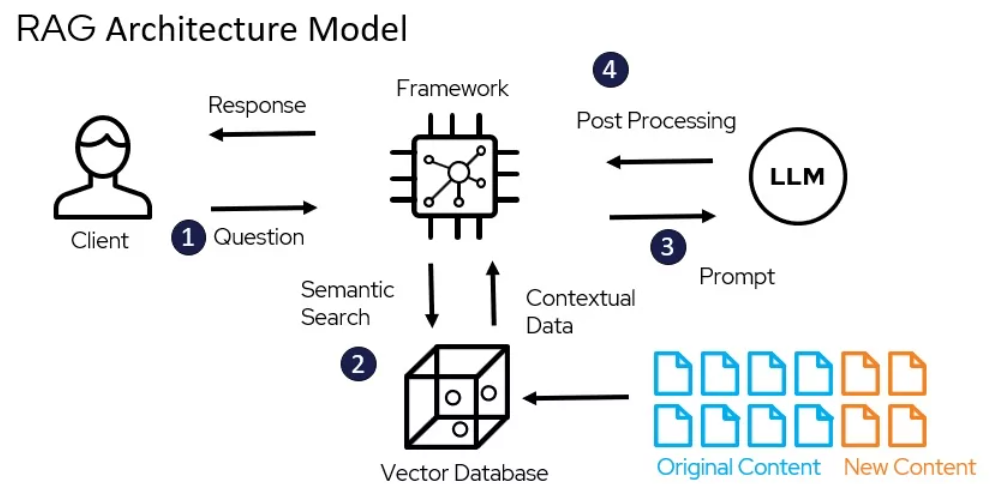
\includegraphics[width=0.8\textwidth]{archivos/RAG_scheme.png} % Ajusta el ancho como necesites
    \caption[Esquema de un sistema RAG]{Esquema visual del funcionamiento de un sistema RAG, mostrando el flujo desde la consulta del usuario, pasando por la recuperación de información relevante, hasta la generación de la respuesta final por el LLM.}
    \label{fig:rag_scheme} % Etiqueta para referenciar la figura en el texto
\end{figure}
\bigskip % Añade un poco de espacio vertical después de la figura

\subsection{Justificación del Proyecto}
El objetivo principal de este \gls{tfg} es proponer una solución a un problema muy común que es la necesidad de acceder a la información de forma rápida, fácil y precisa. Es una experiencia generalizada la frustración que sale de no encontrar un archivo importante, una fotografía específica o un documento entre la inmensa cantidad de datos que se suelen acumular.

Los métodos tradicionales para la búsqueda de archivos presentan limitaciones significativas. Por un lado, las búsquedas basadas únicamente en metadatos, como nombres de archivo, fechas o etiquetas asignadas manualmente, resultan muchas veces ineficaces ya que dependen de una organización previa meticulosa y de la capacidad del usuario para recordar dichos detalles. Por otro lado, la búsqueda directa de contenido bruto, es decir, la localización de una palabra o frase exacta dentro de los ficheros, puede ser un proceso lento, especialmente con grandes volúmenes de archivos. Además, este enfoque tiende a generar un alto número de resultados irrelevantes (falsos positivos) y su aplicabilidad se restringe principalmente a documentos textuales, excluyendo imágenes, vídeos y otros formatos de archivo.

En este contexto surge la propuesta de este proyecto, el desarrollo de un sistema inteligente de búsqueda de archivos. El objetivo es permitir a los usuarios localizar la información deseada mediante consultas formuladas en lenguaje natural, es decir, utilizando sus propias palabras, de manera similar a como interactuarían con otra persona. Para lograrlo, se emplearán modelos de \gls{ia} con capacidad para comprender diversos tipos de archivos (multimodales), no solo texto, lo que permitirá la creación de un índice basado en el significado semántico real de su contenido. Adicionalmente, se implementará una arquitectura de tipo \gls{rag}. Se espera que esta combinación facilite la recuperación de la información más pertinente y su presentación de forma útil para el usuario.

Es importante recalcar que la ejecución de un proyecto de estas características es, en la actualidad, técnicamente viable, incluso para su implementación en ordenadores personales. Los avances recientes han propiciado la disponibilidad de \gls{gpu} progresivamente más potentes y accesibles. De forma paralela, han emergido modelos de \gls{ia} más compactos y eficientes, como los modelos ligeros o cuantizados descritos anteriormente, capaces de realizar tareas complejas, como la comprensión del lenguaje natural, sin requerir recursos computacionales masivos. Este panorama posibilita que este tipo de búsqueda inteligente deje de ser exclusiva de grandes corporaciones y se convierta en una herramienta al alcance de cualquier usuario.

Si bien existen herramientas que emplean \gls{ia} para la búsqueda de información, como Perplexity AI (orientada a la web) o ciertas funcionalidades de búsqueda integradas en aplicaciones específicas, este proyecto se distingue por su enfoque en la búsqueda inteligente y multimodal \textit{dentro del repositorio de archivos personales del usuario}, en su propio dispositivo o sistema de almacenamiento local. Mientras numerosas soluciones se concentran en entornos en la nube o en datos de dominio público, la iniciativa LLMSearch pretende ofrecer una herramienta privada y eficiente para la gestión del universo digital individual. Esto permitirá la localización de contenido en imágenes, documentos y otros formatos basándose en su semántica, y no exclusivamente en palabras clave o metadatos. La idea es trasladar la potencia de los \gls{llm} y la búsqueda semántica directamente al entorno de escritorio del usuario, haciendo que la interacción con su propia información sea más sencilla y cómoda.

\subsection{Repositorio del proyecto}
El código fuente del proyecto, junto con la documentación y ejemplos de uso, está disponible en el siguiente repositorio de GitHub: \url{https://github.com/Nekoraru22/TFG-LLMSearch}. Este repositorio incluye las instrucciones para la instalación y ejecución de todo el sistema.